\documentclass[conference]{IEEEtran}

\usepackage{graphicx}
\usepackage{booktabs}
\usepackage{array}
\usepackage{hyperref}
\usepackage{xcolor}
\usepackage{tikz}
\usetikzlibrary{arrows.meta, positioning, shapes.geometric}
\hypersetup{
    colorlinks=true,
    linkcolor=black,
    urlcolor=black,
    citecolor=black
}

% Screenshot helper for IEEE double-column layout:
% Usage: \screenshotfigure{image-path}{height}{caption}{label}
% Replace only the image path when adding your final screenshots.
% The image stays inside one column using \linewidth.
\newcommand{\screenshotfigure}[4]{
\begin{figure}[!t]
\centering
\IfFileExists{#1}{
    \includegraphics[width=\linewidth,height=#2,keepaspectratio]{#1}
}{
    \fbox{\parbox[c][#2][c]{0.92\linewidth}{\centering
    \textbf{Screenshot Placeholder}\\[0.15cm]
    Add the correct screenshot image path in the LaTeX code.}}
}
\caption{#3}
\label{#4}
\end{figure}
}

\begin{document}

% =========================
% COVER PAGE
% =========================
\begin{titlepage}
    \centering
    \vspace*{0.45cm}

    \IfFileExists{figures/bahria-logo.png}{
        \includegraphics[width=0.3\textwidth]{figures/bahria-logo.png}\\[0.35cm]
    }{
        \vspace*{0.45cm}
    }

    {\Large \textbf{BAHRIA UNIVERSITY}\par}
    \vspace{0.08cm}
    {\large Islamabad Campus\par}
    \vspace{0.08cm}
    {\large Department of Computer Science\par}

    \vspace{0.7cm}

    \vspace{0.35cm}
    {\Large \textbf{AIL 201 -- Artificial Intelligence Lab}\par}
    \vspace{0.12cm}

    {\large Final Project Report\par}
    \vspace{0.35cm}


    \vspace{0.4cm}
    {\Huge \textbf{EarthScan AI}\par}
    \vspace{0.3cm}
    {\Large \textbf{Building Damage Assessment from Pre/Post Satellite Images}\par}
    \vspace{0.18cm}
    {\large Using CNN and CNN+KNN Models\par}

    \vspace{0.95cm}
    \renewcommand{\arraystretch}{1.18}
    \begin{tabular}{>{\bfseries}p{3.6cm}p{8.4cm}}
        Domain & Artificial Intelligence, Computer Vision, Disaster Damage Assessment \\
        Course Code & AIL 201 \\
        Semester & \textbf{[BS CS 5(A)]} \\
        Submitted To & \textbf{[Ma'am Laiba Gull]} \\
        Submission Date & \textbf{[May 18,2026]} \\
    \end{tabular}
    \renewcommand{\arraystretch}{1.0}

    \vspace{1.05cm}
    {\large \textbf{Group Members}\par}
    \vspace{0.28cm}
    \renewcommand{\arraystretch}{1.25}
    \begin{tabular}{p{4.2cm}p{3.1cm}p{4.7cm}}
        \toprule
        \textbf{Name} & \textbf{Roll Number} & \textbf{Main Contribution} \\
        \midrule
        \textbf{[Hadia Cheema]} & \textbf{[01-134232-056]} & Models, Reasearch, Report \\
        \textbf{[Umm e Habiba Imran]} & \textbf{[01-134241-048]} & Frontend, Testing, Documentation \\
        \textbf{[Zainab Idrees]} & \textbf{[01-134241-051]} & Dataset, Backend, Evaluation \\
        \bottomrule
    \end{tabular}
    \renewcommand{\arraystretch}{1.0}


\end{titlepage}

\title{\LARGE \textbf{EarthScan AI: Building Damage Assessment from Pre/Post Satellite Images Using Hybrid CNN and KNN Techniques}}


\maketitle

\begin{abstract}
Disaster damage assessment is a time-sensitive computer vision problem because affected buildings must be identified quickly after events such as floods, storms, earthquakes, and fires. This report presents EarthScan AI, a desktop web-based artificial intelligence application for classifying building damage from paired pre-disaster and post-disaster satellite images. The system uses the xBD/xView2 disaster dataset and predicts four image-level damage classes: no damage, minor damage, major damage, and destroyed. A Python Flask backend performs image preprocessing, loads trained machine learning models, and returns predictions through a web interface. Two models are implemented and evaluated: a Siamese CNN using a MobileNetV2-based feature extractor and a hybrid CNN+KNN pipeline. The final evaluation was performed over five runs using accuracy, precision, recall, and F1-score with mean and standard deviation. The application also includes confidence charts, Matplotlib evaluation graphs, and a visual-change heatmap to support result interpretation.
\end{abstract}

\begin{IEEEkeywords}
building damage assessment, satellite imagery, xBD, xView2, convolutional neural network, K-nearest neighbors, Flask, computer vision, disaster response.
\end{IEEEkeywords}

\section{Summary}
Natural disasters can damage buildings over wide geographic areas, making manual assessment slow and difficult. Satellite imagery provides a practical way to observe affected regions before and after a disaster. The goal of this project is to develop an AI-based system that can accept a pre-disaster and post-disaster satellite image pair and predict the overall building damage severity.

EarthScan AI uses paired satellite images as input and produces meaningful output through a web interface. The backend preprocesses both images, combines them into a six-channel input, and sends them to trained CNN and CNN+KNN models. The expected outcome is a predicted damage class with confidence values, comparison between models, and supporting visualizations for the user.

This project satisfies the AI Lab requirement of a working Python-based backend, trained ML model, functional web interface, dataset description, numerical evaluation, Matplotlib visualizations, and GitHub-ready source code structure.

\section{Technologies Used}
Table~\ref{tab:tech} lists the major technologies used in the project.

\begin{table}[h]
\centering
\caption{Technologies and Tools Used}
\label{tab:tech}
\begin{tabular}{p{2.2cm}p{5.2cm}}
\toprule
\textbf{Category} & \textbf{Technology} \\
\midrule
Language & Python, HTML, CSS, JavaScript \\
Backend & Flask, Flask-CORS \\
ML/DL & TensorFlow/Keras, Scikit-learn, Joblib \\
Image Processing & OpenCV, NumPy \\
Visualization & Matplotlib, Chart.js \\
Dataset & xBD / xView2 Challenge Dataset \\
Interface & Desktop web-based GUI \\
Version Control & GitHub public repository \\
\bottomrule
\end{tabular}
\end{table}

\section{Dataset Description}
The dataset used in this project is the xBD/xView2 disaster damage assessment dataset. It contains satellite images captured before and after disasters, along with JSON annotations describing building damage levels. The labeled training portion was used to create paired samples by matching image IDs.

Each sample contains:
\begin{itemize}
    \item One pre-disaster RGB satellite image.
    \item One matching post-disaster RGB satellite image.
    \item One image-level damage label selected from post-disaster annotations.
\end{itemize}

The final processed dataset contains 2,799 labeled pre/post image pairs. The split used for model training and evaluation is shown in Table~\ref{tab:split}.

\begin{table}[h]
\centering
\caption{Train, Validation, and Test Split}
\label{tab:split}
\begin{tabular}{lcc}
\toprule
\textbf{Split} & \textbf{Samples} & \textbf{Ratio} \\
\midrule
Training & 1,959 & 70\% \\
Validation & 420 & 15\% \\
Testing & 420 & 15\% \\
\bottomrule
\end{tabular}
\end{table}

The damage classes are no damage, minor damage, major damage, and destroyed. The input shape after preprocessing is \(256 \times 256 \times 6\). Channels 0--2 contain the pre-disaster RGB image, while channels 3--5 contain the post-disaster RGB image.

\subsection{Preprocessing Steps}
The preprocessing pipeline includes:
\begin{enumerate}
    \item Matching pre-disaster and post-disaster images using the same image ID.
    \item Reading images using OpenCV.
    \item Converting BGR images to RGB.
    \item Resizing each image to \(256 \times 256\).
    \item Normalizing pixel values to the range [0, 1].
    \item Concatenating pre and post images into a six-channel array.
    \item Applying stratified train, validation, and test split.
\end{enumerate}

\subsection{Sample Dataset Row}
\begin{table}[h]
\centering
\caption{Example Dataset Row}
\label{tab:sample}
\begin{tabular}{p{2.4cm}p{5cm}}
\toprule
\textbf{Field} & \textbf{Example} \\
\midrule
Pair ID & hurricane-michael\_00000004 \\
Pre Image & hurricane-michael\_00000004\_pre\_disaster.png \\
Post Image & hurricane-michael\_00000004\_post\_disaster.png \\
Label & major-damage / destroyed / etc. \\
Input Shape & \(256 \times 256 \times 6\) \\
\bottomrule
\end{tabular}
\end{table}

\section{ML Model Explanation}
Two model approaches were implemented and compared.

\subsection{CNN Model}
The CNN model uses a Siamese-style architecture. The six-channel input is split into pre-disaster and post-disaster RGB images. Both images are passed through a shared MobileNetV2-based feature extractor. Temporal difference features are computed and combined with pre and post features. The final dense layers classify the image pair into one of four damage classes.

This model fits the problem because convolutional neural networks are effective for extracting spatial features from image data, while the paired input allows the model to learn before-and-after disaster changes.

\subsection{CNN+KNN Model}
The CNN+KNN model uses the CNN as a feature extractor. Features from the dense layer named \texttt{features} are extracted and passed to a KNN classifier with distance weighting. This hybrid approach compares deep features using a classical machine learning classifier.

This method is useful for the AI Lab project because it demonstrates both deep learning and traditional ML classification in one application.

\subsection{Training Process}
Training was performed with data augmentation enabled only for the training split. Validation and test images were not augmented. Class weights were used to reduce the effect of class imbalance. The final evaluation used five independent runs with different random seeds.

\section{System Architecture}
Fig.~\ref{fig:architecture} shows the system architecture and data flow.

\begin{figure}[h]
\centering
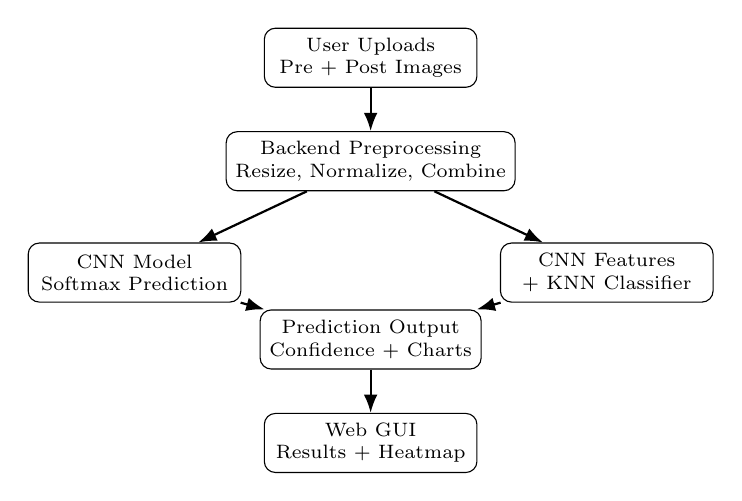
\begin{tikzpicture}[
    node distance=0.55cm,
    block/.style={rectangle, draw, rounded corners, align=center, minimum width=2.7cm, minimum height=0.75cm, font=\scriptsize},
    arrow/.style={-{Latex}, thick}
]
\node[block] (input) {User Uploads\\Pre + Post Images};
\node[block, below=of input] (preprocess) {Backend Preprocessing\\Resize, Normalize, Combine};
\node[block, below left=0.65cm and -0.2cm of preprocess] (cnn) {CNN Model\\Softmax Prediction};
\node[block, below right=0.65cm and -0.2cm of preprocess] (knn) {CNN Features\\+ KNN Classifier};
\node[block, below=1.5cm of preprocess] (output) {Prediction Output\\Confidence + Charts};
\node[block, below=of output] (gui) {Web GUI\\Results + Heatmap};
\draw[arrow] (input) -- (preprocess);
\draw[arrow] (preprocess) -- (cnn);
\draw[arrow] (preprocess) -- (knn);
\draw[arrow] (cnn) -- (output);
\draw[arrow] (knn) -- (output);
\draw[arrow] (output) -- (gui);
\end{tikzpicture}
\caption{System architecture showing input, preprocessing, model prediction, output, and GUI flow.}
\label{fig:architecture}
\end{figure}

\section{Screenshots}
This section includes placeholders for the required running application screenshots. Replace only the image paths below with the final screenshot file paths before submission. These figures are adjusted for the IEEE double-column format, so each screenshot appears inside one report column.

\screenshotfigure
{figures/pre_post.png}
{4.3cm}
{Input screen where the user uploads pre-disaster and post-disaster satellite images.}
{fig:ss-upload}


\screenshotfigure
{figures/newresults.png}
{4.3cm}
{Output screen showing CNN and CNN+KNN predictions, confidence values, comparison chart, and visual-change heatmap.}
{fig:ss-result}

\screenshotfigure
{figures/evaluationnew.png}
{4.1cm}
{About or evaluation screen showing Matplotlib visualizations such as five-run mean and standard deviation, training curve, and confusion matrices.}
{fig:ss-about-visualizations}

\textbf{Recommended screenshots to add:}
\begin{itemize}
    \item Upload tab with both image upload boxes visible.
    \item Loading/processing screen after clicking Analyze Damage.
    \item Results tab showing predictions, confidence chart, and heatmap.
    \item About tab showing Matplotlib evaluation visualizations, if space allows.
\end{itemize}

\section{Results and Evaluation}
The final model was evaluated using five runs. Each run used 10 epochs, batch size 16, and training-only augmentation. The metrics include accuracy, precision, recall, and F1-score. The final mean and standard deviation are shown in Table~\ref{tab:results}.

\begin{table}[h]
\centering
\caption{Final 5-Run Evaluation Results}
\label{tab:results}
\begin{tabular}{lcccc}
\toprule
\textbf{Model} & \textbf{Acc.} & \textbf{Prec.} & \textbf{Recall} & \textbf{F1} \\
\midrule
CNN & 67.10$\pm$1.73 & 67.81$\pm$3.10 & 67.10$\pm$1.73 & 66.51$\pm$2.48 \\
CNN+KNN & 69.14$\pm$2.84 & 66.57$\pm$3.43 & 69.14$\pm$2.84 & 67.10$\pm$3.07 \\
\bottomrule
\end{tabular}
\end{table}

The CNN+KNN approach achieved the best average accuracy, so the best run from the final evaluation, run 02, was selected for backend deployment. The backend uses the trained CNN model, CNN feature extractor, and KNN classifier from run 02.

\begin{figure}[h]
\centering
\includegraphics[width=\linewidth]{figures/5runnew.png}
\caption{Matplotlib chart showing five-run mean and standard deviation for CNN and CNN+KNN.}
\label{fig:meanstd}
\end{figure}

\begin{figure}[h]
\centering
\includegraphics[width=\linewidth]{figures/trainingnew.png}
\caption{Training and validation accuracy/loss curve for selected backend run 02.}
\label{fig:traincurve}
\end{figure}

\begin{figure}[h]
\centering
\includegraphics[width=\linewidth]{figures/confusionmatrixnew.png}
\caption{CNN+KNN confusion matrix for selected backend run 02 on the test split.}
\label{fig:cm}
\end{figure}

\subsection{Heatmap Note}
The heatmap included in the web application is a visual-change map. Red and yellow regions indicate high visual change between pre and post images, green and cyan indicate moderate change, and blue or purple indicate low change. This heatmap is not pixel-level damage segmentation; the final damage class is predicted by the trained CNN and CNN+KNN models.

\section{GitHub Link}
The complete source code, README file, requirements file, backend, frontend, and final evaluation files will be uploaded to a public GitHub repository.

\vspace{0.2cm}
\noindent\textbf{GitHub Repository:} 
\begin{enumerate}
    \item \url{https://github.com/zainabidrees1234/EarthScan_AI_BuildingDamagePredictor.git}\\
    \item \url{https://github.com/fitbit12/EarthScanAI}\\
    \item \url{https://github.com/habiba-imran/EarthScan-AI}
\end{enumerate}




\vspace{0.2cm}
\noindent\textbf{Kaggle Dataset Link:} \\
\url{https://www.kaggle.com/datasets/tunguz/xview2-challenge-dataset-train-and-test/data}

\vspace{0.2cm}
\noindent\textbf{Processed Dataset Artifact & Model Artifact:} \\
\url{https://drive.google.com/drive/folders/1jO6sM5ITwhpdJQgm1GqR2TbwZUswZLKB?dmr=1&ec=wgc-drive-%5Bmodule%5D-goto}


\vspace{0.2cm}
\noindent\textbf{Note:} The raw dataset, processed NumPy arrays in \texttt{processed\_balanced\_pairs\_256/}, and trained model binaries are too large for regular GitHub upload. Therefore, the GitHub repository contains the source code, frontend/backend, README, requirements file, scripts, report, and small result visualizations. Large dataset/model artifacts should be downloaded from the provided external links and placed in the same folder structure before retraining or full reproduction.

\section{Conclusion}
EarthScan AI successfully demonstrates an applied artificial intelligence solution for building damage assessment using paired pre-disaster and post-disaster satellite imagery. The project fulfills the main requirements of the AI Lab final project by including a trained machine learning model, a Python-based backend, a functional desktop web interface, meaningful user input and output, Matplotlib visualizations, and five-run evaluation results with mean and standard deviation.

The system uses two approaches: a CNN model and a hybrid CNN+KNN model. The CNN learns visual features from the combined six-channel pre/post image input, while the CNN+KNN approach uses CNN-extracted features for distance-based classification. The final results show that the CNN+KNN model achieved the best average accuracy among the evaluated models, making it suitable for backend deployment in the web application.

Overall, the project provides a complete workflow from dataset preprocessing and augmentation to model training, evaluation, backend integration, and frontend result display. Although the heatmap is not a pixel-level damage segmentation map, it adds useful visual support by highlighting areas of strong visual change between the two input images. In future work, the system can be improved by using larger training data, more advanced deep learning architectures, object-level building localization, and true segmentation-based damage maps.

\end{document}
